%%%%%%%%%%%%%%%%%%%%%%%%%%%%%%%%%%%%%%%%%
% Jacobs Landscape Poster
% LaTeX Template
% Version 1.1 (14/06/14)
%
% Created by:
% Computational Physics and Biophysics Group, Jacobs University
% https://teamwork.jacobs-university.de:8443/confluence/display/CoPandBiG/LaTeX+Poster
% 
% Further modified by:
% Nathaniel Johnston (nathaniel@njohnston.ca)
%
% This template has been downloaded from:
% http://www.LaTeXTemplates.com
%
% License:
% CC BY-NC-SA 3.0 (http://creativecommons.org/licenses/by-nc-sa/3.0/)
%
%%%%%%%%%%%%%%%%%%%%%%%%%%%%%%%%%%%%%%%%%

%----------------------------------------------------------------------------------------
%	PACKAGES AND OTHER DOCUMENT CONFIGURATIONS
%----------------------------------------------------------------------------------------

\documentclass[final]{beamer}

\usepackage[scale=1.24]{beamerposter} % Use the beamerposter package for laying out the poster

\usetheme{confposter} % Use the confposter theme supplied with this template

\setbeamercolor{block title}{fg=ngreen,bg=white} % Colors of the block titles
\setbeamercolor{block body}{fg=black,bg=white} % Colors of the body of blocks
\setbeamercolor{block alerted title}{fg=white,bg=dblue!70} % Colors of the highlighted block titles
\setbeamercolor{block alerted body}{fg=black,bg=dblue!10} % Colors of the body of highlighted blocks
% Many more colors are available for use in beamerthemeconfposter.sty

%-----------------------------------------------------------
% Define the column widths and overall poster size
% To set effective sepwid, onecolwid and twocolwid values, first choose how many columns you want and how much separation you want between columns
% In this template, the separation width chosen is 0.024 of the paper width and a 4-column layout
% onecolwid should therefore be (1-(# of columns+1)*sepwid)/# of columns e.g. (1-(4+1)*0.024)/4 = 0.22
% Set twocolwid to be (2*onecolwid)+sepwid = 0.464
% Set threecolwid to be (3*onecolwid)+2*sepwid = 0.708

\newlength{\sepwid}
\newlength{\onecolwid}
\newlength{\twocolwid}
\newlength{\threecolwid}
\setlength{\paperwidth}{48in} % A0 width: 46.8in
\setlength{\paperheight}{36in} % A0 height: 33.1in
\setlength{\sepwid}{0.024\paperwidth} % Separation width (white space) between columns
\setlength{\onecolwid}{0.22\paperwidth} % Width of one column
\setlength{\twocolwid}{0.464\paperwidth} % Width of two columns
\setlength{\threecolwid}{0.708\paperwidth} % Width of three columns
\setlength{\topmargin}{-0.5in} % Reduce the top margin size
%-----------------------------------------------------------

\usepackage{graphicx}  % Required for including images

\usepackage{booktabs} % Top and bottom rules for tables
\usepackage{tikz}
\usepackage{dirtytalk}
\usepackage{mdframed}


%----------------------------------------------------------------------------------------
%	TITLE SECTION 
%----------------------------------------------------------------------------------------

\title{Event Ordering of News Articles}% Poster title

\author{James Friel} % Author(s)

\institute{Supervisor: Shay Cohen} % Institution(s)

%----------------------------------------------------------------------------------------

\begin{document}
\addtobeamertemplate{headline}{} 
{\begin{tikzpicture}[remember picture, overlay]
     \node [anchor=north east, inner sep=3cm]  at (current page.north east)
     {
\includegraphics[height=5cm]{logo.jpg}};
  \end{tikzpicture}}
\addtobeamertemplate{block end}{}{\vspace*{2ex}} % White space under blocks
\addtobeamertemplate{block alerted end}{}{\vspace*{2ex}} % White space under highlighted (alert) blocks

\setlength{\belowcaptionskip}{2ex} % White space under figures
\setlength\belowdisplayshortskip{2ex} % White space under equations

\begin{frame}[t] % The whole poster is enclosed in one beamer frame

\begin{columns}[t] % The whole poster consists of three major columns, the second of which is split into two columns twice - the [t] option aligns each column's content to the top

\begin{column}{\sepwid}\end{column} % Empty spacer column

\begin{column}{\onecolwid} % The first column

%----------------------------------------------------------------------------------------
%	OBJECTIVES
%----------------------------------------------------------------------------------------

  \begin{alertblock}{Objectives}
    The aim of this thesis is to construct a system that predicts the most probable path
    through an edge-weighted directional graph of events.
    we aim to construct this graph by extracting data from Wikipedia for each event and
    build a date estimate from Wikipedia. From this data we will conduct several experiments
    to maximise the likely-hood of a graph traversal.
  
\end{alertblock}

%----------------------------------------------------------------------------------------
%	INTRODUCTION
%----------------------------------------------------------------------------------------

\begin{block}{Introduction}
Nominal data is descriptive in nature, making is difficult to assign an Canonical ordering to.
The problem tackled in this dissertation is the ordering of news article headlines to generate
a most-probable traversal of a weighted directed graph of these events.
This problem is based off of the paper \cite{abend2015lexical} and some
techniques discussed and used henceforth are based off of this paper.


Our data comes from the Wikipedia ``Today in History'' data set and the nominal data is retrieved
from Wikipedia articles.
\vspace{6cm}
\begin{figure}
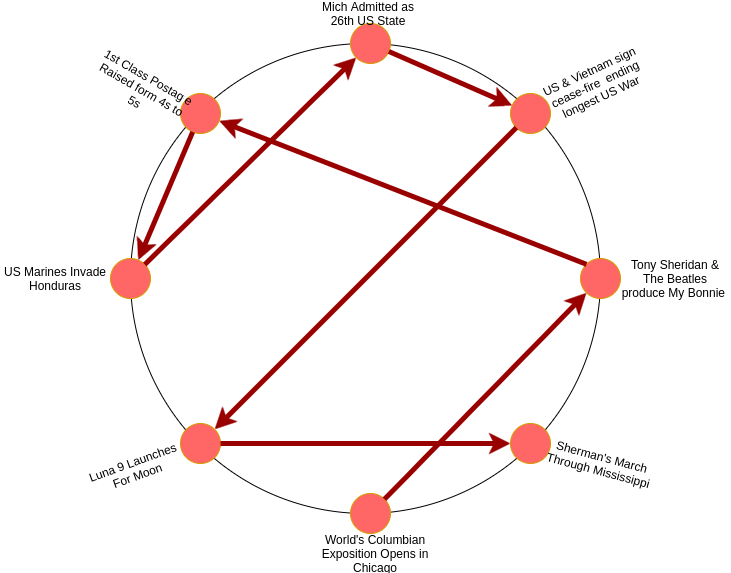
\includegraphics[]{node-graph.png}
\caption{A Graph of the predicted ordering}
\label{node_graph}
\end{figure}

\end{block}

%------------------------------------------------


%----------------------------------------------------------------------------------------

\end{column} % End of the first column

\begin{column}{\sepwid}\end{column} % Empty spacer column

\begin{column}{\twocolwid} % Begin a column which is two columns wide (column 2)

\begin{columns}[t,totalwidth=\twocolwid] % Split up the two columns wide column

\begin{column}{\onecolwid}\vspace{-.6in} % The first column within column 2 (column 2.1)

%----------------------------------------------------------------------------------------
%	MATERIALS
%----------------------------------------------------------------------------------------

  \begin{block}{Wikipedia As a Data Source}

    Wikipedia was chosen as the data source for the project as it has over 40 million
    articles \cite{} and maintains an unbiased presence through community moderating.
    
Using Wikipedia's article retrieval API, gathering the data from
the site is trivial. Choosing what to extract is, however, not
so straightforward.

Using a modified version of Stanfords natural language processing suite,
we are able to build features from out data.

Using this toolkit, the Open Information Extraction from
The University of Washington is used to extract Subjects, Objects
and their relations from our event titles.

\end{block}

%----------------------------------------------------------------------------------------

\end{column} % End of column 2.1

\begin{column}{\onecolwid}\vspace{-.6in} % The second column within column 2 (column 2.2)

%----------------------------------------------------------------------------------------
%	METHODS
%----------------------------------------------------------------------------------------

\begin{block}{Classification}
  Given that each event in our data set is of the form
  \begin{equation}
  (t_{i},d_{i}) \hspace{0.5em}for\hspace{0.5em} i \epsilon [M],
    \end{equation}
    where t is the title, d is the associated date and M is the original data set,
    we constructed a new data set
    \begin{equation}
      \{(t_{i},s_{i},d_{j})\} \hspace{0.5em} for \hspace{0.5em}i,j [M]
    \end{equation}
    This will form the basis of our data to generate features.

    From this we built a new data set
    \begin{equation}
      \{(t_{i},s_{i},t_{j},s_{j},b_{ij})\} \hspace{0.5em} for \hspace{0.5em} i,j \epsilon [M]
      \end{equation}
where $b_{ij} = [y_{i} > y_{j}]$ indicating which event came first.
A similar data set was constructed using only the article headlines.

With this new data set we began to experiment with techniques to classify a test set of the data. 
%SVMs, Perceptrons, Logistics Regression and Multi-Layered Perceptrons were experimented with, amongst other techniques.
\end{block}

%----------------------------------------------------------------------------------------

\end{column} % End of column 2.2

\end{columns} % End of the split of column 2 - any content after this will now take up 2 columns width

%----------------------------------------------------------------------------------------
%	IMPORTANT RESULT
%----------------------------------------------------------------------------------------

\begin{alertblock}{Important Result}
  \begin{center}
  The use of external data sources, such as Wikipedia, greatly improves the ability to order\\ saline events in chronological order.
  \end{center}
\end{alertblock} 

%----------------------------------------------------------------------------------------

\begin{columns}[t,totalwidth=\twocolwid] % Split up the two columns wide column again

\begin{column}{\onecolwid} % The first column within column 2 (column 2.1)

%----------------------------------------------------------------------------------------
%	MATHEMATICAL SECTION
%----------------------------------------------------------------------------------------

\begin{block}{Graphing}
  From our classifier we produce a complete digraph.
  In order to construct the most likely path through this graph we must solve a variation of
  the travelling salesman problem.
  \vspace{1em}
  
  \begin{mdframed}
    Starting from any node, find the node that will
    generate the most probable path through  every
    other node without visiting any node twice.
\end{mdframed}

  \vspace{1em}

  We solve this problem by using the minimum spanning path algorithm whilst inverting the edge weights
  of the graph. The results of which can be seen in Figure \ref{node_graph}
\end{block}

%----------------------------------------------------------------------------------------

\end{column} % End of column 2.1

\begin{column}{\onecolwid} % The second column within column 2 (column 2.2)

%----------------------------------------------------------------------------------------
%	RESULTS
%----------------------------------------------------------------------------------------

\begin{block}{Results}


\begin{table}[H]
\centering
\label{table:local-learning}
\begin{tabular}{|p{5em}|l|l|l|p{4em}|}
  \hline
  {\small Accuracy}  & {\small DT* (tuple)} & {\small DT* (triple)} & {\small SVM}  & {\small Logistic Regression}\\
  \hline
{\small With Articles}    & 53\%  & 48\%    & 66\% &  76\% \\
\hline
{\small With Titles} & 43\%  & 36& 51\%    & 52\% \\
\hline
\end{tabular}
\caption{\tabular[t]{@{}l@{}}Local Learning Results  \\*DT = Decision Tree \endtabular}
\end{table}

\begin{table}[H]
\centering
\label{table:global-learning}
\begin{tabular}{|p{5em}|l|l|p{4em}|}
  \hline
  {\small Accuracy}  & {\small Perceptron} & {\small MLP}\\
  \hline
{\small With Articles}    & 66\%  & 83\%\\
\hline
{\small With Titles} & 46\%  & 54\%\\
\hline
\end{tabular}
\caption{Global Learning Results}
\end{table}



\end{block}

%----------------------------------------------------------------------------------------

\end{column} % End of column 2.2

\end{columns} % End of the split of column 2

\end{column} % End of the second column

\begin{column}{\sepwid}\end{column} % Empty spacer column

\begin{column}{\onecolwid} % The third column

%----------------------------------------------------------------------------------------
%	CONCLUSION
%----------------------------------------------------------------------------------------

\begin{block}{Conclusion}
  As we can see from the results, the addition of external data sources greatly aids in
  automatic ordering of saline events.

\end{block}

%----------------------------------------------------------------------------------------
%	ADDITIONAL INFORMATION
%----------------------------------------------------------------------------------------

\begin{block}{Future Work}
If I was to take this project forward, there would be a several things I would look into
\begin{itemize}
\item The use of news websites as data sources
\item The use of DNNs in classification
\item Improved Graphing Techniques
\end{itemize}

\end{block}

%----------------------------------------------------------------------------------------
%	REFERENCES
%----------------------------------------------------------------------------------------

\begin{block}{References}

%\nocite{*} % Insert publications even if they are not cited in the poster
\small{\bibliographystyle{unsrt}
\bibliography{references}\vspace{0.75in}}

\end{block}

%----------------------------------------------------------------------------------------
%	ACKNOWLEDGEMENTS
%----------------------------------------------------------------------------------------

\setbeamercolor{block title}{fg=red,bg=white} % Change the block title color

\begin{block}{Acknowledgements}
  I would like to thank Shay Cohen for all of the advice and guidance given during the project.\\
  I would also like to thank Greggs Bakery for  helping me survive through coffee and morning rolls.

\end{block}

%----------------------------------------------------------------------------------------
%	CONTACT INFORMATION
%----------------------------------------------------------------------------------------

\setbeamercolor{block alerted title}{fg=black,bg=norange} % Change the alert block title colors
\setbeamercolor{block alerted body}{fg=black,bg=white} % Change the alert block body colors

\begin{alertblock}{Contact Information}

  \begin{itemize}
    \item Web: \href{http://jamesfriel.uk}{jamesfriel.uk}
    \item Email: \href{mailto:s1332298@ed.ac.uk}{s1332298@ed.ac.uk}
\end{itemize}

\end{alertblock}

\begin{center}
\begin{tabular}{ccc}
\end{tabular}
\end{center}

%----------------------------------------------------------------------------------------

\end{column} % End of the third column

\end{columns} % End of all the columns in the poster

\end{frame} % End of the enclosing frame

\end{document}
